% Setup -------------------------------

\documentclass[a4paper]{report}
\usepackage[a4paper, total={6in, 10in}]{geometry}
\setcounter{secnumdepth}{3}
\setcounter{tocdepth}{3}

\usepackage{titlepic}

\usepackage{hyperref}
\usepackage{indentfirst}

\usepackage{graphicx}
\usepackage{subcaption}
\usepackage[export]{adjustbox}
\usepackage{float}

% Encoding
%--------------------------------------
\usepackage[T1]{fontenc}
\usepackage[utf8]{inputenc}
%--------------------------------------

% Portuguese-specific commands
%--------------------------------------
\usepackage[portuguese]{babel}
%--------------------------------------

% Hyphenation rules
%--------------------------------------
\usepackage{hyphenat}
%--------------------------------------

% References (BibTeX)
%--------------------------------------
\usepackage[backend=bibtex,style=numeric,sorting=ynt]{biblatex}
\usepackage[autostyle=true]{csquotes}
\addbibresource{Report.bib}
%--------------------------------------

% Capa do relatório

\title{
	Sistemas Distribuídos em Larga Escala
	\\ \Large{\textbf{Trabalho Prático}}
	\\ -
	\\ Mestrado em Engenharia Informática
	\\ Universidade do Minho
}
\author{
	\begin{tabular}{ll}
		\textbf{Grupo}
		\\
		\hline
		PG41080 & João Ribeiro Imperadeiro
        \\
		PG41081 & José Alberto Martins Boticas
		\\
        PG41091 & Nelson José Dias Teixeira
	\end{tabular}
	\vspace{1cm}
}

\date{31 de maio de 2020}

\titlepic{
	\vspace{2cm}
	
\includegraphics[scale=0.065]{Images/EEUM_logo.png}
}

\begin{document}

\begin{titlepage}
    \maketitle
\end{titlepage}

\tableofcontents

% Introdução

\chapter{Introdução} \label{ch:Introduction}
\large{
	O presente relatório descreve o desenvolvimento do projeto de cariz prático da unidade curricular de Sistemas Distribuídos em Larga Escala.
	Neste trabalho é requerida a implementação de um dos algoritmos de agregação distribuída disponíveis no documento de suporte ao enunciado do mesmo \parencite{article}.
	Após a implementação do algoritmo escolhido, é posteriormente solicitado o teste do mesmo no simulador desenvolvido ao longo do semestre do presente ano letivo.

	A agregação de dados distribuídos desempenha um papel bastante importante na concepção de diversos sistemas escaláveis uma vez que possibilita a determinação descentralizada de propriedades globais significativas, 
	que posteriormente podem ser utilizadas para direcionar a execução de outras aplicações distribuídas.
	Vários algoritmos de agregação distribuída foram propostos ao longo dos últimos anos, exibindo propriedades diferentes em termos de precisão, 
	desempenho e de métricas de comunicação. No entanto, muitas dessas abordagens não possuem caraterísticas relacionadas com a tolerância de faltas. 
	Desta forma, este grupo de trabalho viu-se interessado em implementar um dos algoritmos com esta propriedade, \textit{flow updating} \parencite{ref}.

	Relativamente à estrutura deste relatório, é exibido o algoritmo escolhido, apresentando o conceito e a implementação intrínsecos ao mesmo. 
	Para além disso, são evidenciados alguns aspetos relativos ao simulador utilizado para proceder à realização de testes do algoritmo em causa, efetuando-se posteriormente uma análise dos resultados obtidos.
	Por fim, são resumidos os tópicos referentes a este trabalho, concluindo, assim, a sua realização.
}

{\let\clearpage\relax \chapter{Algoritmo} \label{ch:Algorithm}}
\large{
	O algoritmo \textbf{\textit{flow updating}}, ao nível de comunicação, é classificado como não estruturado, inserindo-se na categoria \textit{gossip} que, por sua vez, diz respeito à forma como as mensagens são disseminadas pela rede de comunicação.
	Quanto à perspetiva computacional, este algoritmo tem como objetivo a computação iterativa de médias parciais que, ao longo do tempo, convergem.
	Esta última técnica permite também a derivação de outras funções de agregação (como por exemplo, \textit{count} ou \textit{sum}), de acordo com as combinações dos valores inicialmente instanciados.

	Uma das razões que levou este grupo a escolher este algoritmo foi a capacidade do mesmo em tolerar a injeção de faltas transientes. 
	Esta última caraterística é bastante importante sobretudo no que diz respeito à perda de mensagens trocadas na rede de comunicação.
	Com pequenas alterações, é ainda possível que o algoritmo suporte falhas de membros e falhas permanentes de ligações.
	Para além destas vantagens associadas ao contexto de sistemas distribuídos, este algoritmo possui não só um melhor desempenho quando comparado com os outros da mesma classe, como também possibilita uma computação mais precisa de valores.
	Por fim, a execução do algoritmo em causa é independente da topologia do roteamento de rede.

	No \hyperref[ch:Analysis of results]{4º capítulo} deste documento são devidamente clarificados todos os resultados obtidos após a implementação do algoritmo escolhido, discutindo-se a veracidade das propriedades mencionadas acima.

	\section{Conceito} \label{sec:Concept}
	O algoritmo \textit{flow updating} difere de outros propostos para o mesmo problema no sentido em que não se procede ao envio de mensagens complexas que, posteriormente, são armazenadas e disseminadas.
	Em contraste, faz uso do conceito de fluxo (no sentido da teoria de grafos), atualizando-o com recurso ao valor inicial e à contribuição de fluxos de outros nós vizinhos, sendo que o fluxo é simétrico nos extremos de cada ligação. Por isto, a soma das médias de cada um dos nós deve manter-se constante.
	Assim, partilha-se apenas o fluxo com os vizinhos, sendo que a perda de uma destas mensagens não implica uma falha grave.
	A intuição é que a simetria pode ser quebrada, se for possível garantir que uma mensagem chegará no futuro e a restabeleça.

	Importa realçar que existem duas versões do algoritmo. A primeira assenta no envio de mensagens com recurso a \textit{broadcast} (\textit{N} para \textit{N}) enquanto que a segunda enquadra-se no envio de mensagens em \textit{unicast} (1 para 1).


	\section{Implementação} \label{sec:Implementation}
	Tal como foi referido no fim do \hyperref[sec:Concept]{subcapítulo anterior}, foram implementadas duas versões distintas do algoritmo em questão.
	À semelhença do que foi elaborado durantes as aulas práticas desta unidade curricular, estas duas versões foram implementadas na linguagem \texttt{Python}.
	Para cada uma das mesmas são exibidos os respetivos detalhes computacionais.

		\subsection{\textit{Broadcast}} \label{subsec:Broadcast}
		Relativamente a esta abordagem, criou-se uma classe para representar um nó do grafo, com o nome \texttt{flowUpdatingBroadcast}, que contém as seguintes informações no seu estado:
		\begin{itemize}
			\item um dicionário \textit{f} que contém os fluxos desses nós para os seus vizinhos;
			\item um dicionário \textit{e} que contém as estimativas que recebeu dos seus vizinhos;
			\item o seu valor inicial \textit{v};
			\item a lista dos seus vizinhos;
			\item as mensagens acumuladas de uma ronda;
			\item um inteiro \textit{timeout} que representa a duração pré-estabelecida de cada ronda.
		\end{itemize}

		Esta classe contém ainda as seguintes funções:
		\begin{itemize}
			\item \texttt{gen\_message} - devolve a lista de mensagens a serem enviadas nessa ronda, incluindo uma mensagem especial de \textit{timeout}, dirigida ao próprio nó e que representa o fim de uma ronda;
			\item \texttt{state\_transition} - executada em reação à mensagem de \textit{timeout}, ou seja, no fim da ronda, por forma a calcular as novas estimativas e fluxos dos vizinhos, bem como os próprios;
			\item \texttt{calculate\_estimate} - executada pelo método anterior e que corresponde ao valor calculado durante a transição de estado, ou seja, devolve a nova estimativa para o valor objetivo.
		\end{itemize}

		\subsection{\textit{Unicast}} \label{subsec:Unicast}
		Quanto a esta versão, concebeu-se, da mesma forma, uma classe para representar um nó do grafo, com o nome \texttt{flowUpdatingUnicast}, que contém as mesmas informações, no seu estado, que as indicadas acima, para a classe de \textit{Broadcast}.
		Para além destas, têm ainda um inteiro representativo do identificador do vizinho escolhido, sendo que o mesmo é selecionado pela função \texttt{chooseNeighbor}, que, tal como o nome transparece, devolve aleatoriamente o identificador de um dos vizinhos.

		As funções desta classe são as mesmas que as expostas anteriormente na classe \textit{broadcast}, com as seguintes alterações:
		\begin{itemize}
			\item \texttt{gen\_message} - calcula apenas uma mensagem para o vizinho \textit{k}, em vez de todos os vizinhos, e a mensagem especial de fim de ronda;
			\item \texttt{state\_transition} - calcula apenas a estimativa e o fluxo do vizinho \textit{k};
		\end{itemize}
}

{\let\clearpage\relax \chapter{Simulador} \label{ch:Simulator}}
\large{
	O simulador presente neste projeto consiste num programa escrito em \texttt{Python} que modela um sistema distribuído composto por um número arbitrário de nós e respetivas ligações entre eles.
	Para além disso, este simula a passagem de tempo, permitindo não só a injeção de faltas através da eliminação de mensagens como também possibilita a mudança de vizinhança.
	
	Para poder simular um sistema composto por vários nós, este guarda no seu estado uma lista com os nós do sistema e as distâncias de todas as ligações que existem. Para além disto, tem uma lista onde guarda as mensagens pendentes do sistema e um inteiro que representa o tempo atual (numa unidade arbitrária).
	
	De forma a ser possível costumizar o comportamento da simulação, podem ser configurados diversos parâmetros, entre os quais a probabilidade de falha no envio de uma mensagem, a periodicidade em que ocorrem mudanças de vista (isto é, a alteração das ligações do sistema) e, ainda, o \textit{timeout} que é utilizado para o envio de mensagens periódicas de um nó para ele mesmo (representa, por exemplo, o fim de uma ronda).
	
	Para ajustar ao algoritmo selecionado, tivemos de implementar um mecanismo de deteção da precisão da estimativa atual dos nós do grafo gerado, por forma a garantir que o algoritmo converge corretamente.
	Para isso, foi desenvolvida uma forma de computar o valor alvo (\textit{target}) para que, posteriormente, este seja comparado com a estimativa momentânea de todos os nós. No caso de haver uma aproximação com um erro inferior a 0.01, dá-se por concluída a execução do algoritmo.

	Quanto aos métodos que o simulador possui, temos a destacar:
	\begin{itemize}
		\item \texttt{start} - gera as mensagens iniciais, calcula o valor objetivo e programa a primeira mudança de vista, no caso desta existir;
		\item \texttt{runLoop} - processa as mensagens do sistema, tratando não só de entregá-las ao seu destino como também de incorporar as novas. Para além disso, é responsável pelas mudanças de vista e injeção de faltas, bem como a terminação do algoritmo no caso do valor objetivo ser atingido (dentro da margem de erro estipulada);
		\item \texttt{closeToTarget} - verifica se a estimativa do sistema está suficientemente próxima do valor objetivo.
	\end{itemize}

	Assim, foi possível averiguar a natureza inerente ao algoritmo \textit{flow updating}, observando-se o seu comportamento no âmbito de sistemas distribuídos.
}

{\let\clearpage\relax \chapter{Análise de resultados obtidos} \label{ch:Analysis of results}}
\large{
	Em relação às duas variantes deste algoritmo, verificou-se que a versão \textit{broadcast} é melhor do que a \textit{unicast} em termos do número de rondas e de mensagens trocadas.
	O número de rondas apresenta uma maior descrepância entre as duas versões, o que é explicável pelo facto de na versão \textit{broadcast} cada nó enviar mensagens para todos os vizinhos em cada ronda, 
	enquanto na versão \textit{unicast} cada nó envia apenas um mensagem para um vizinho a cada ronda.	
	É também de salientar que mesmo em condições de perdas significativas de mensagens, o algoritmo elegido exibe um desempenho satisfatório, convergindo sempre para o valor pretendido.

	Nos gráficos em que podemos ver a relação entre o número de nós e o número de mensagens/rondas temos algumas flutuações em relação aos resultados que esperávamos.
	Tal pode ser explicado por serem criados grafos novos para cada número diferente de nós, sendo que, por ser seguido um método aleatório na geração das ligações do grafo, 
	o número de ligações ou até mesmo o diâmetro do grafo, podem ter influência no tempo de execução do algoritmo.
	Nos gráficos que relacionam a percentagem de mensagens perdidas com o número de mensagens/rondas as mesmas flutuações já não existem, uma vez que o grafo utilizado é sempre o mesmo.

	Exibem-se de seguida 4 gráficos que evidenciam a respetiva análise:
	\begin{figure}[H]
		\centering
		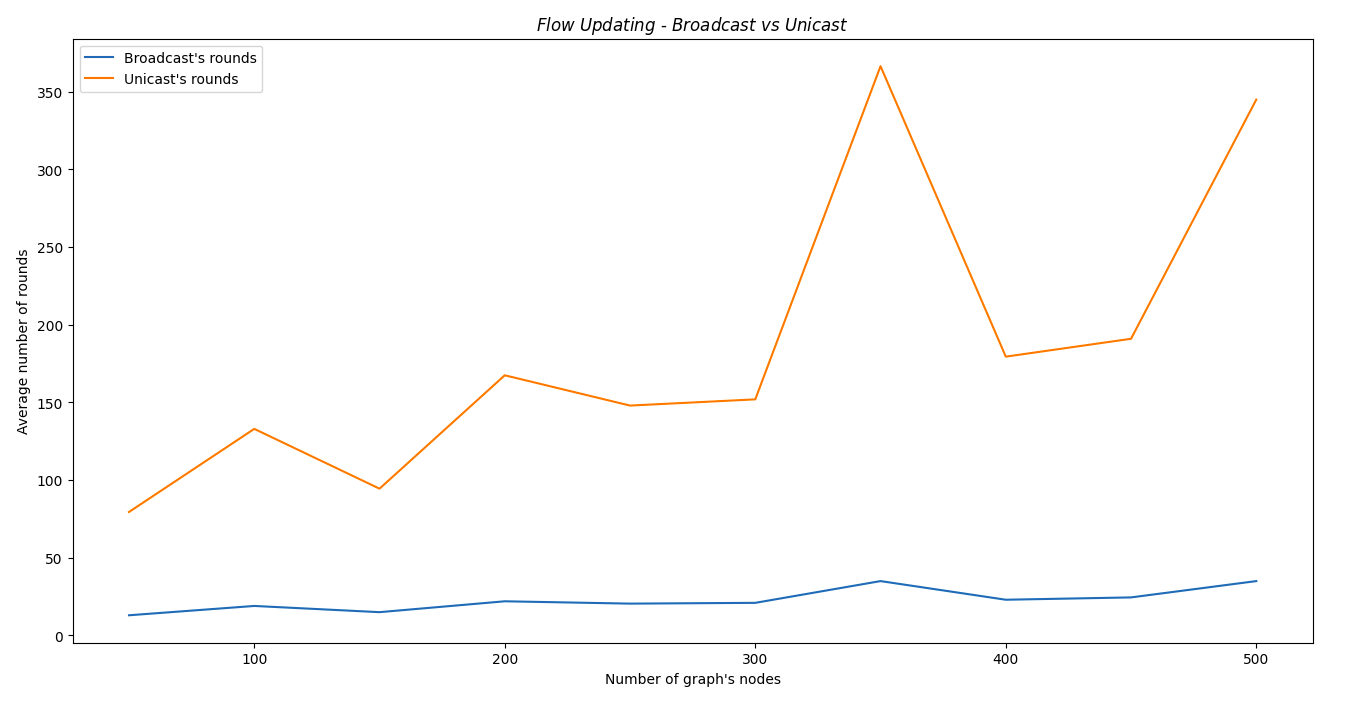
\includegraphics[width=0.99\textwidth]{Images/Plot1.png}
		\label{fig:1}
	\end{figure}
	
	\begin{figure}[H]
		\centering
		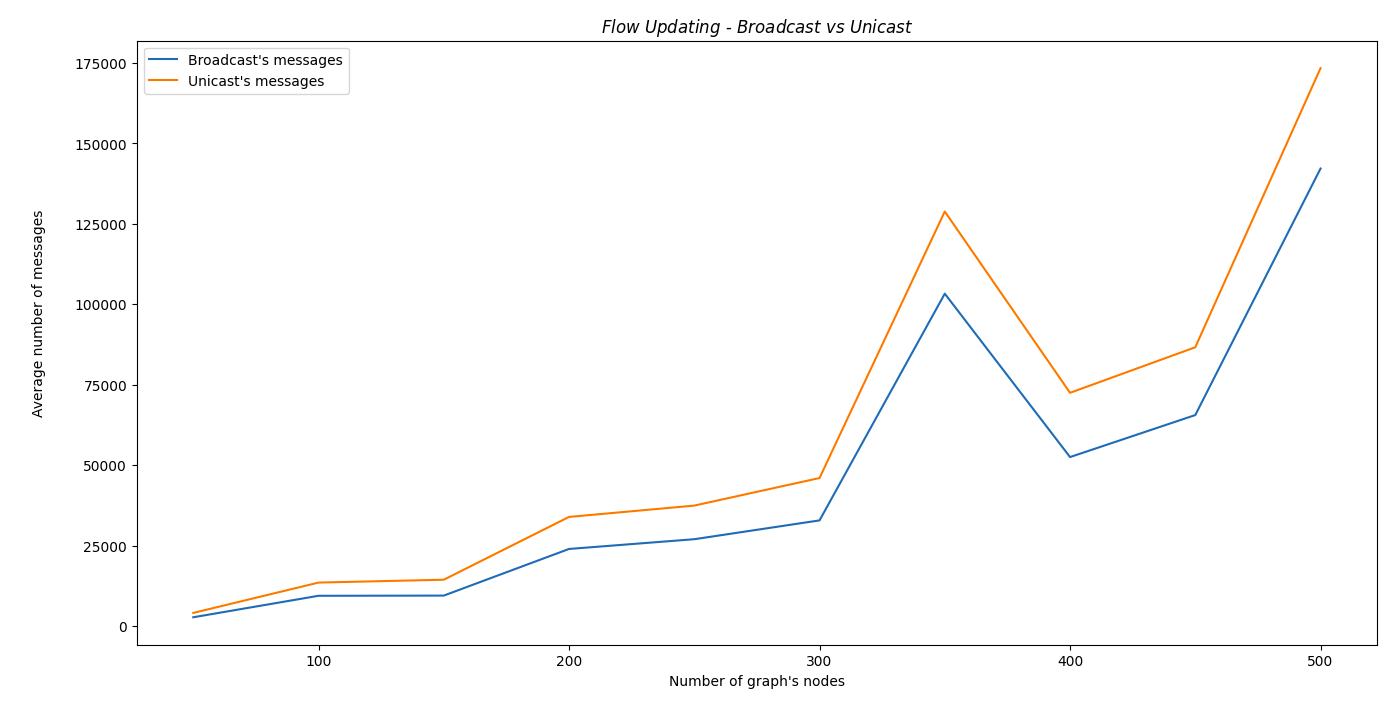
\includegraphics[width=0.99\textwidth]{Images/Plot2.png}
		\label{fig:2}
	\end{figure}

	\begin{figure}[H]
		\centering
		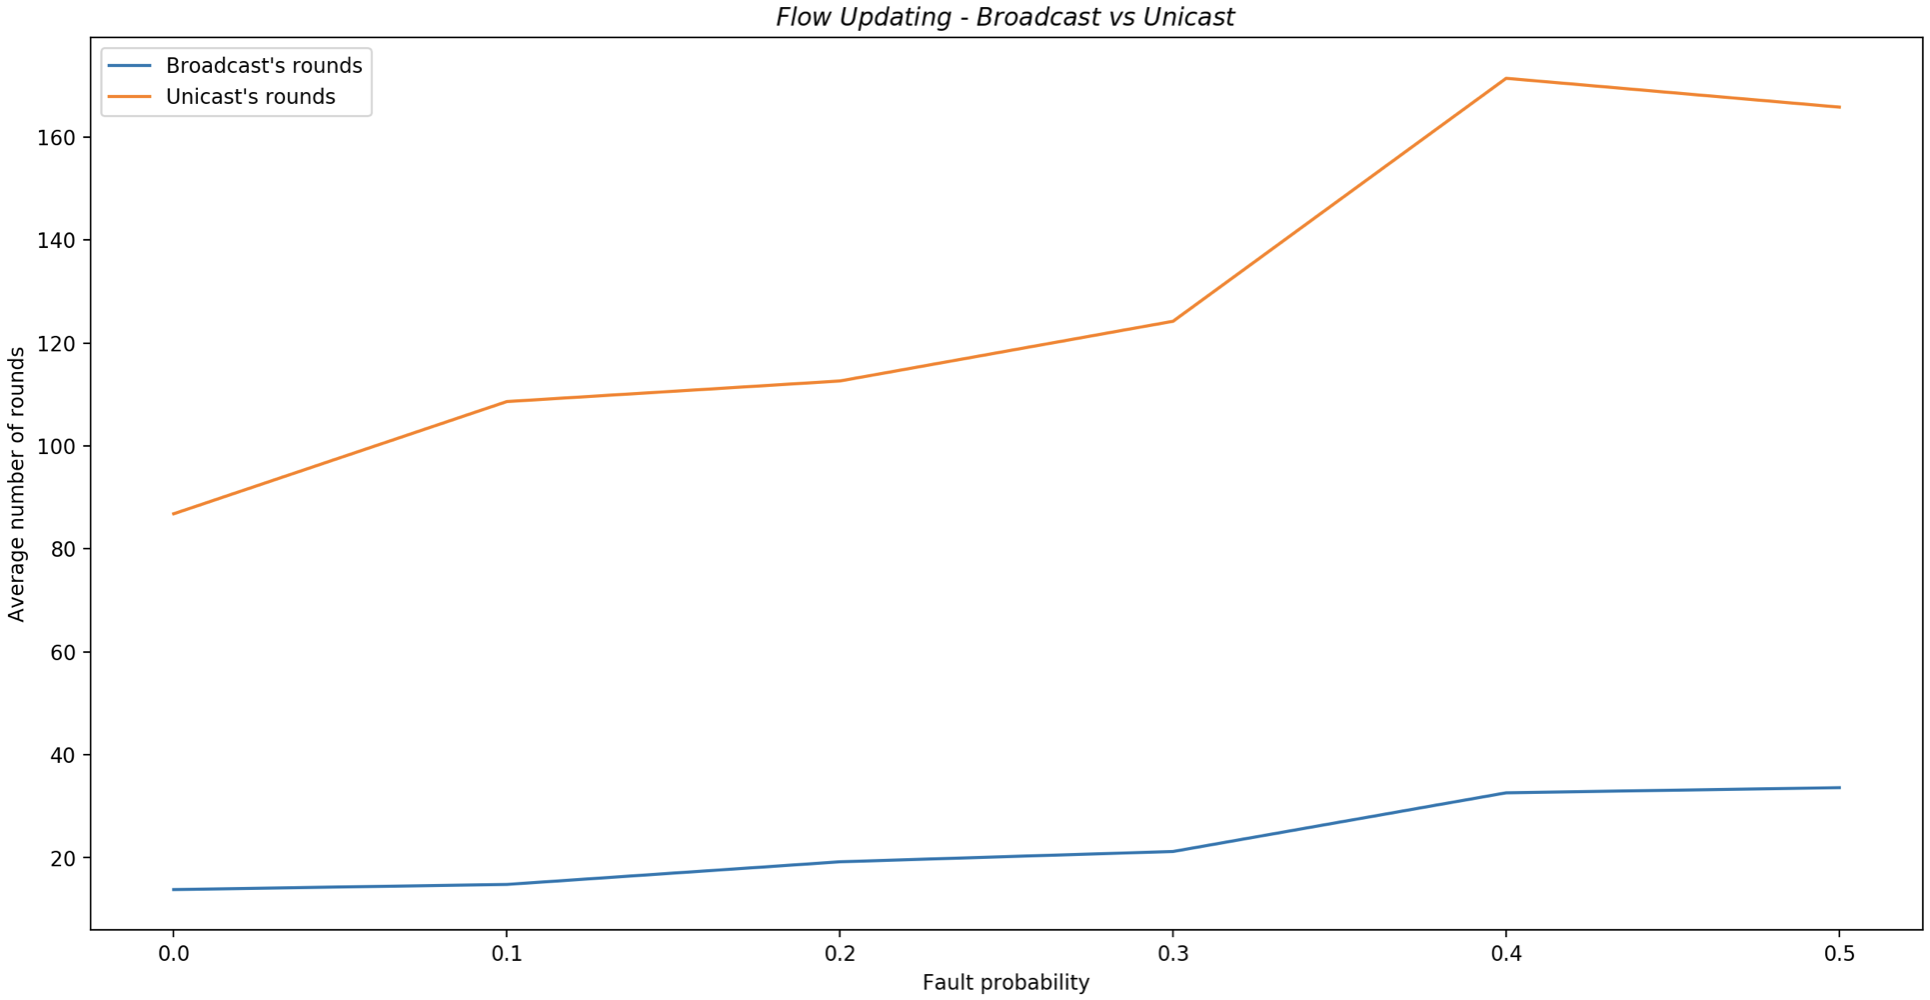
\includegraphics[width=0.99\textwidth]{Images/Plot3.png}
		\label{fig:3}
	\end{figure}

	\begin{figure}[H]
		\centering
		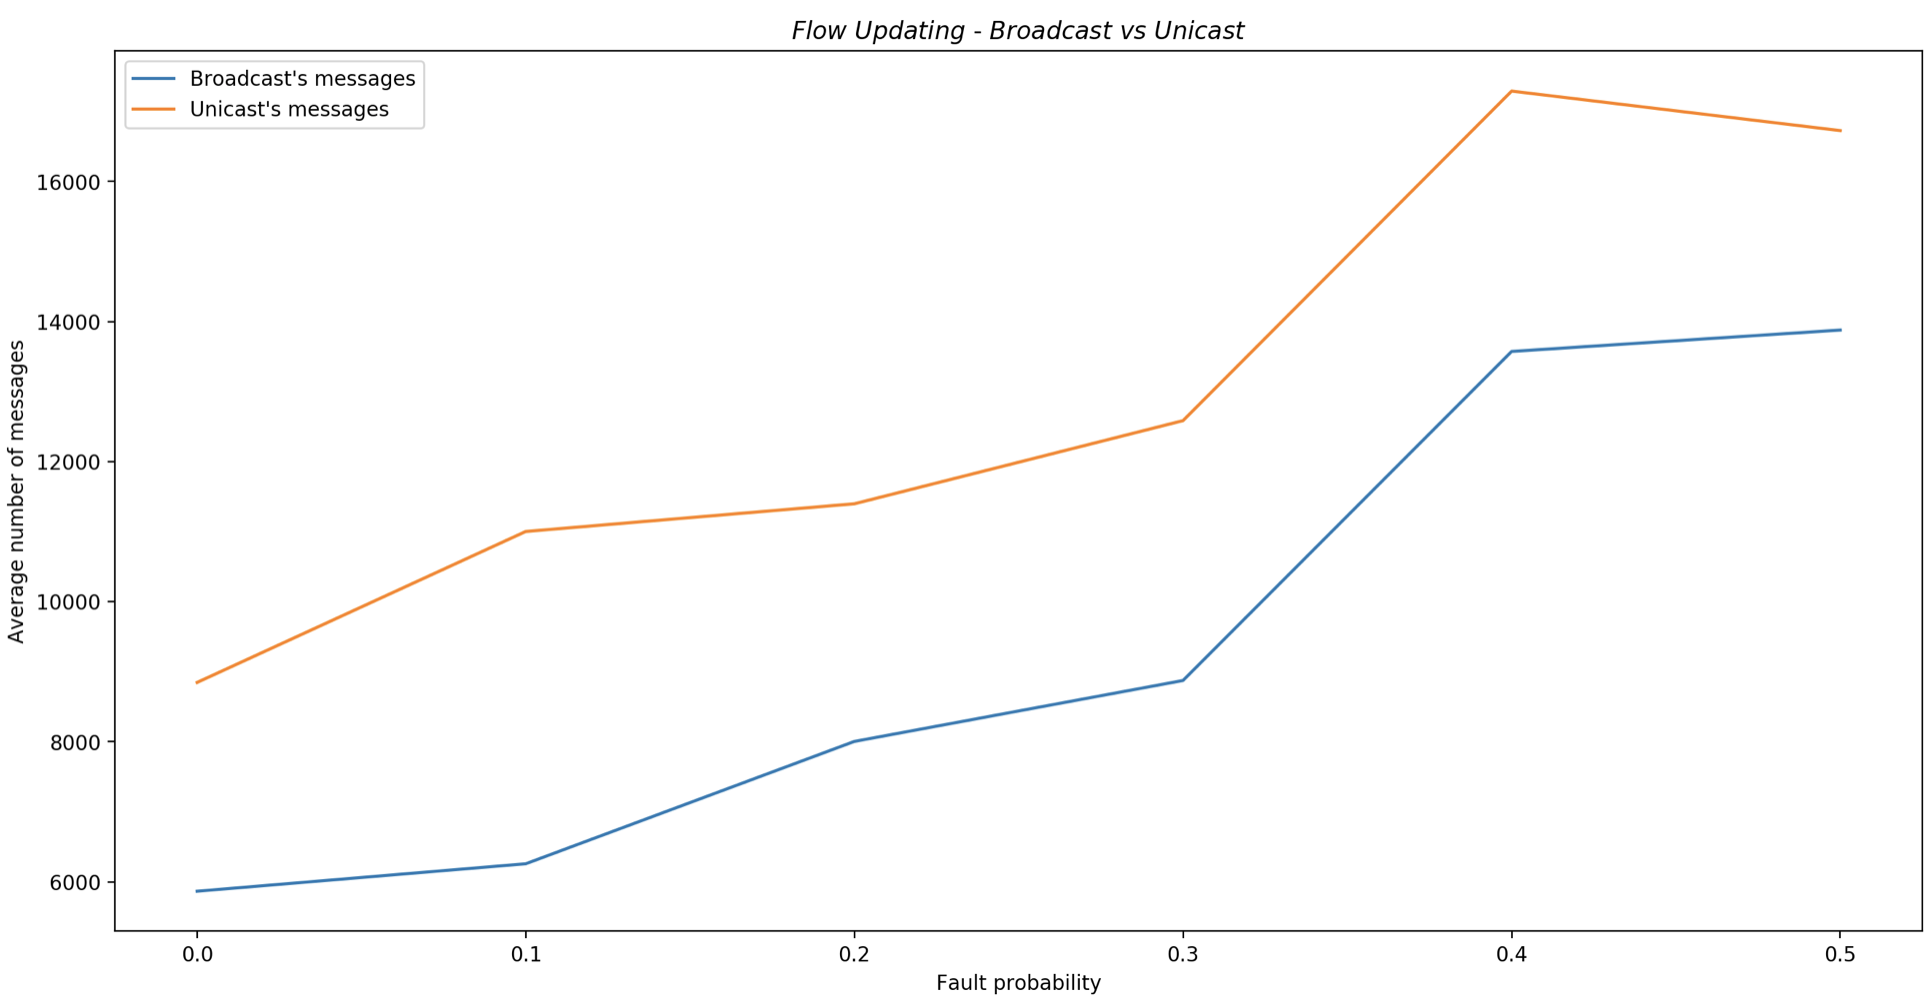
\includegraphics[width=0.99\textwidth]{Images/Plot4.png}
		\label{fig:4}
	\end{figure}
}

{\let\clearpage\relax \chapter{Conclusão} \label{ch:Conclusion}}
\large{
	Apesar do algoritmo selecionado por este grupo de trabalho trocar um maior número de mensagens na rede de comunicação (ainda que pouco significativo) do que outros de agregação distribuída, \textit{flow updating} é a única abordagem robusta e resiliente de agregação tolerante a falhas conhecida.
	Esta é capaz de se adaptar continuamente às mudanças topológicas da rede, sem recorrer a nenhum tipo de mecanismo de reinicialização. Além disso, este algoritmo é adequado em cenários dinâmicos, onde são necessárias estimativas precisas sem haver a imposição muito restrita ao nível da quantidade de mensagens trocadas.
	Durante a implementação do algoritmo, o simulador ajudou na conceção do mesmo, uma vez que foi possível tirar ilações enquanto este era desenvolvido. 
	Também permitiu encontrar erros, testar o algoritmo, comparar versões, testar otimizações e implementá-las.
	No geral, o desempenho do simulador e do algoritmo são satisfatórios, o que nos permite afirmar que atingimos os objetivos propostos.
}

\printbibliography[heading=bibintoc]

\end{document}